% Created 2023-01-19 Thu 15:54
% Intended LaTeX compiler: lualatex
\documentclass[11pt]{article}
\usepackage{graphicx}
\usepackage{longtable}
\usepackage{wrapfig}
\usepackage{rotating}
\usepackage[normalem]{ulem}
\usepackage{amsmath}
\usepackage{amssymb}
\usepackage{capt-of}
\usepackage{hyperref}
\usepackage[margin=0.5in]{geometry}
\author{David Lewis}
\date{1/17/2022}
\title{Lec 4: Classroom activity}
\hypersetup{
 pdfauthor={David Lewis},
 pdftitle={Lec 4: Classroom activity},
 pdfkeywords={},
 pdfsubject={},
 pdfcreator={Emacs 28.2 (Org mode 9.6)}, 
 pdflang={English}}
\begin{document}

\maketitle
\section*{1.}
\label{sec:org065bafd}
\subsection*{a.}
\label{sec:orgb099e59}
4 * 0.1\textsuperscript{2} = 0.04 = 4\% = 1/25
\subsection*{b.}
\label{sec:orgf71ce7e}
\(2^d \cdot \epsilon^d\) where \(\epsilon \le 0.1\)
\subsection*{c.}
\label{sec:org82b3e3b}
\begin{itemize}
\item \((2 \cdot \epsilon) \le 0.2\)
\item \((2\epsilon)^d \rightarrow 0\) as d trends toward \(\infty\)
\end{itemize}
\subsection*{d.}
\label{sec:orgdf76e36}
\begin{itemize}
\item \(V = 1 - (1-\epsilon)^d\)
\item volume of unit hypercube is 1
\item volume of inner hypercube is \((1-\epsilon)^d\)
\item volume of inner cube subtracted from outer cube is the volume of the shell
\end{itemize}
\subsection*{e.}
\label{sec:orgdb7ef39}
\begin{itemize}
\item \(1 - (1-\epsilon)^d \rightarrow 0\) as d trends toward \(\infty\) because \(\epsilon \le 0.1\)
\end{itemize}
\section*{2.}
\label{sec:org7500c1d}
\subsection*{a.}
\label{sec:org9153419}
\begin{center}
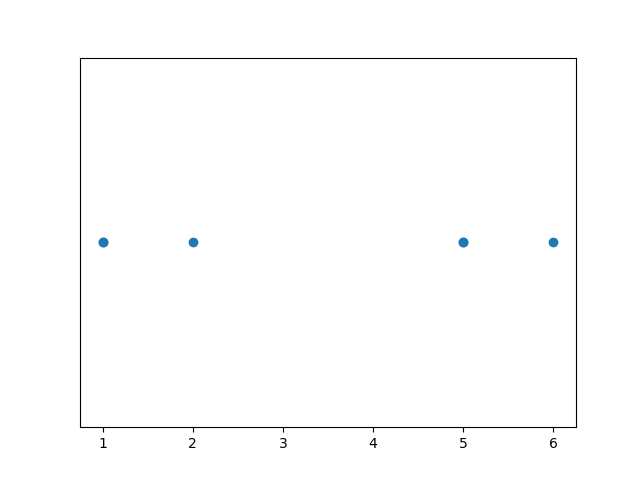
\includegraphics[width=2in]{2a.png}
\end{center}
\subsection*{b.}
\label{sec:orge9e22f9}
\begin{itemize}
\item Diagonal: \((0,0,0)\rightarrow (1, 1, 1)\)
\item Anti-diagonal: \((1, 1, 0) \rightarrow (0,0,1)\)
\end{itemize}
\subsection*{c.}
\label{sec:orgb90da07}
\begin{itemize}
\item \(\theta = \arccos(\frac{(v_1 \cdot v_2)}{\|v_1\| \cdot \|v_2\|})\)
\item Change to standard vector notation
\item \(v_1 = (1,1,1), v_2 = (0-1, 0-1, 1-0)\)
\item \(\theta = \arccos(\frac{(-1 -1 + 1)}{\sqrt{3} \cdot \sqrt{3}}) = 109.47^\circ\)
\end{itemize}
\subsection*{e.}
\label{sec:org697c6af}
\begin{itemize}
\item magnitude is the same for both vectors, equal to d
\item \(v_1 = (1, 1, ...)\)  with dimension d
\item \(v_2 = (-1, -1, ..., 1)\) with dimension d
\item \(v_1 \cdot v_2 = v_2 \cdot v_2\)
\item \(\theta_d = \arccos{(\frac{-(d-2)}{d})\)
\end{itemize}
\subsection*{e.}
\label{sec:orgd15e7c2}
\begin{itemize}
\item Intuitively the angle goes toward 180 degrees
\item Angle increases as dimension increases
\item definition of cos \(\theta\) in higher dimensions goes to 1
\item \(\frac{-(d-2)}{d} \rightarrow 1\) as d goes to \(\infty\)
\item \(\arccos(1) = 180^\circ\)
\end{itemize}
\end{document}
